\begin{document}

\maketitle

\section{Introduction}
\begin{frame}[fragile]
  \frametitle{Previously}
	Get to know each other and discuss strategy in general
	\begin{itemize}
		\item How to get a grade
		\item IT and business strategy, IT impact on business
		\item On systems and software architecture
	\end{itemize}
\end{frame}

\begin{frame}[fragile]
  \frametitle{Today}
		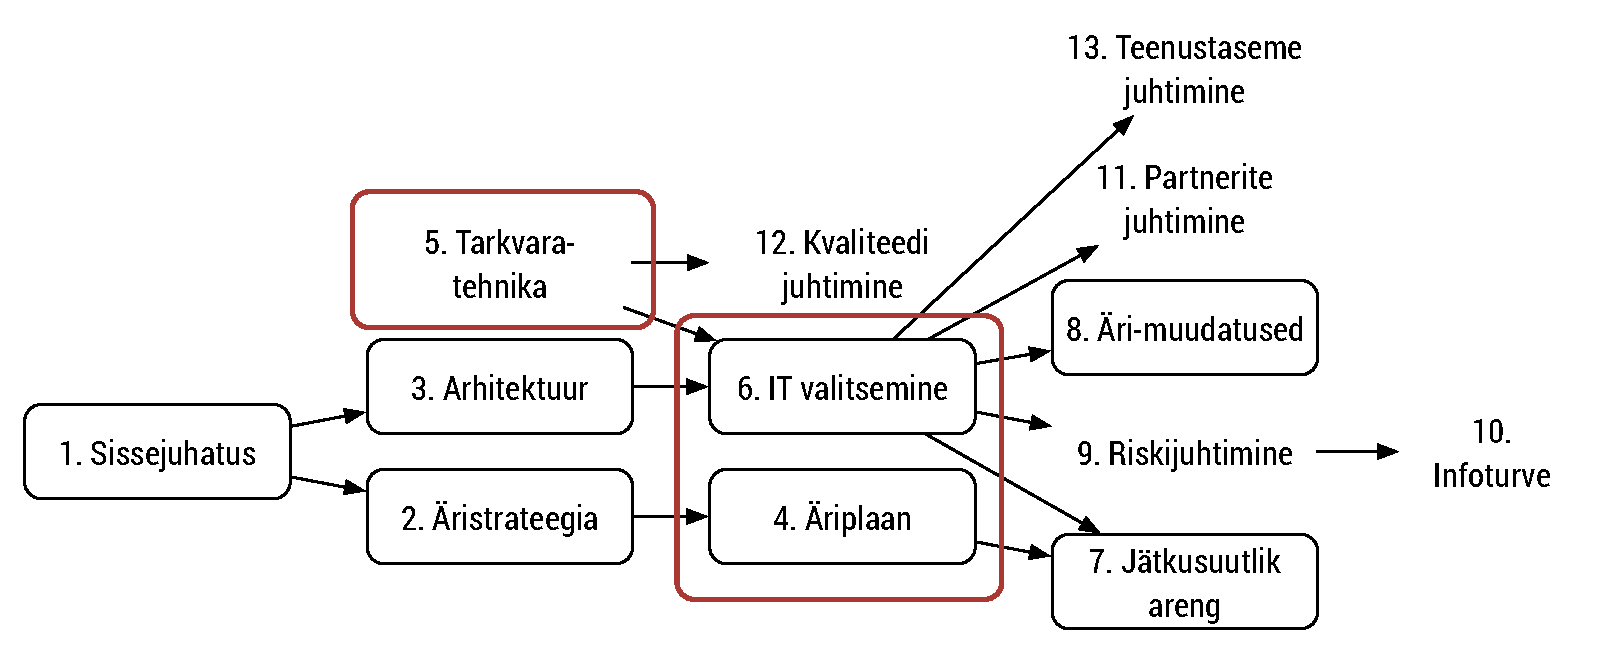
\includegraphics[width=\textwidth]{aine_struktuur_teine.pdf}
\end{frame}

\section{Business planning}
\begin{frame}[fragile]
  \frametitle{IT Expenses}
  	Money is spent on IT only if that spend creates value for shareholders. Thus
	\begin{itemize}
		\item It is entirely normal for the it spend to fluctuate
		\item It is the job of the IT manager to demonstrate how each and every cent spent on IT creates value 
		\note{Not just value but value for stakeholders. Who those stakeholders are and how to they express their concept of value?\\}
		\item The head of IT is to build an IT organisation that corresponds to the business model of the organisation not the other way around
		\note{The tail should not be wagging the dog. This means you have to be able to understand what that business model actually is\\}
	\end{itemize}
\end{frame}

\begin{frame}[fragile]
  \frametitle{Operations and development cost}
			\begin{itemize}
				\item opex is the function of previous opex and \emph{previous devex}
				\item Technical debt stems from the customer and goes to the customer becoming an IT problem in between 
				\item IT value add is often perceived to be via new added functionality
			\end{itemize}
			\begin{center}
\textbf{			Every dollar spent on building new software adds to all future opex}
\\[3mm]
therefore
\\[3mm]
\textbf{With constant total IT spend,\\ the ability of IT to deliver perceived value deteriorates}
			\end{center}
\note{Unless one takes very deliberate steps to both change the perception of value and continuously reduce the cost of maintenance per unit of new functionality. \\}
\end{frame}

\begin{frame}[fragile]
  \frametitle{Conclusions}
	\begin{itemize}
		\item Architecture is a vital function 
		\note{remember the minimising the added complexity per unit of functionality part? \\}
		\item It is strategically important to explain the customer the impact their decisions have on future expenses
		\item Capitalisation decisions are crucial for the IT manager
		\item Therefore the IT manager must be involved in long term financial planning as well as capitalisation decisions
		\note{Fot this to happen, one must be able to contribute to the discussion in a meaningful manner\\}
		\item Technical debt is important
		\note{We'll cover this in more detail in the future\\}
	\end{itemize}
	
	\begin{center}
			\textbf{IT systems are a liability and not an asset}
			\note{An asset is something that gets amortised without incurring an actual cost. A liability incurs a periodic cost}
	\end{center}
\end{frame}


\begin{frame}[fragile]
  \frametitle{Architecture and business}
  \newcommand{\lenitem}[2][.55\linewidth]{\parbox[t]{#1}{\strut #2\strut}}
  
  \mbox{}\hfill\raisebox{-\height}[0pt][0pt]{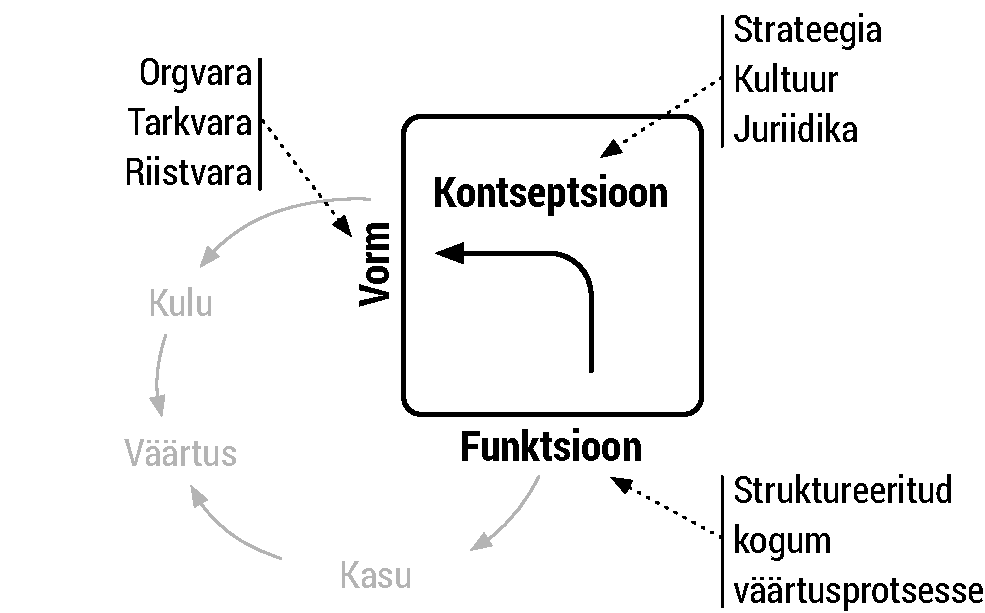
\includegraphics[width=.4\linewidth]{ffc_profit.pdf}}
  \vspace*{-\baselineskip}
  
			\begin{itemize}
				\item \lenitem{Architecture determines the capability of a product or a service to add value}
				\note{Value is defined as benefit at cost\\}
				\item Including
				\begin{itemize}
					\item \lenitem{Opex. Can the ops handle it?}
					\item \lenitem{Manufacturing expensis. How expensive a programmer does our architecture assume?}
					\item Exit cost. How hard it is to get out of the mess?
				\end{itemize}
				\item The architect must fully understand the business model and be capable of doing something with that understanding
			\end{itemize}
\end{frame}
\note{The capability part is important. Good architecture is necessary but not sufficient to turn a profit. Black \& Decker, Volkswagen vs. GM}

%Arutelu koht
\begin{frame}
  \frametitle{Discussion point}
		\begin{center}
			\textbf{How to explain the customer the decisions they made in the past impact the cost base of today?}
		\end{center}
\end{frame}

\section{Software engineering}
\begin{frame}[fragile]
  \frametitle{Software engineering defined}
	\begin{center}
		\begin{quote}
			Software engineering is the application of engineering to the design, development, implementation, testing and maintenance of software in a systematic method
			\note{Basically application of the science of engineering to the world of software.\\Rather good book based on a brief glimpse. Good overview of the topic}
		\end{quote}		
	\end{center}
	\cite{laplante}
\end{frame}

\begin{frame}[fragile]
  \frametitle{Implications of the definition}
	\begin{itemize}
		\item There are seven disciplines mentioned in total. Literally writing code is but one of them
		\note{This is a hint towards general bias: usually we focus on coding and neglect the rest\\}
		\item No particular reference is made towards a development process as such
			\begin{itemize}
				\item The disciplines can be arranged in a variety of ways, which one is the best?
				\note{There is no secret sauce, the particular arrangement depends on your circumstance\\}
				\item The development process gets too much attention in everyday life
				\note{At least in personal experience. Shifting the boxes around is much simpler than trying to get each of the boxes to work properly\\}
			\end{itemize}
		\item Software lifecycle is nicely covered. Software reengineering is part of the lifecycle, is covered in the book and is a significant cost factor
	\end{itemize}
\note{The programmers have kidnapped the software engineering discussion because, although they take up majority of a developers day, they are not nearly as much fun. Programmers are, after all called programmers.}
\end{frame}

\begin{frame}[fragile]
  \frametitle{Importance of software engineering}
  The business strategy is directly linked to the way software is built. Joel \citep{spolsky2004joel2} describes the Amazon vs. Ben \& Jerry's dilemma
  \begin{itemize}
  	\item Organic growth vs. Get Big Fast approach 
	\item Full of good examples of software engineering choices of strategic importance
		  \begin{itemize}
		  	\item Do we solve problems using money or thinking?
			\item How important is the quality of code produced?
			\item Do we pursue sustainable development or are focused on daily firefighting?
		  \end{itemize}
	\item The correct answers depend on your chosen strategy. Therefore
  \end{itemize}
  \begin{center}
	  \textbf{Decide clearly whether you are Amazon or Ben \& Jerry's}
  \end{center}
\end{frame}
\note{Read Joel, he is really really good. Most of the content is freely available on the web but the book is more convenient.\\ Of course, the dilemma presented is but one of the many but nicely illustrates the relationships between software engineering and strategy. \\ The way you build software must support your business strategy, like everything else.}

\begin{frame}[fragile]
  \frametitle{Complexity of building software}
	Brooks says in one of his essays \citep{brooks1975mythical} that \emph{Building software is intrinsically complicated} 
  \begin{itemize}
	\item Through the ages people still have sought the silver bullet 
		  \begin{itemize}
		  	\item Describe the requirements
			\item Use of a (very) particular process
			\item Manufacture of artefacts
			\note{Very widespread in public sector, bureaucrats love producing paper\par}
			\item "Back to the nature" process denial
			\note{This is what is sometimes thought agile is. Quite the contrary}
		  \end{itemize}
	\item So you've got to focus on practical improvements instead of seeking snake-oil
	\note{Remember the definition of software engineering. Focus on making the parts work the best you can and stick them together whichever way feels nice\par
	The rest of Brooks is also very good. "The mythical man-month" should be compulsory reading for anyone who has programmers reporting to them}
  \end{itemize}
\end{frame}


%Arutelu koht
\begin{frame}[fragile]
  \frametitle{Discussion point}
		\begin{center}
			\textbf{What is it that makes programming complex?}
		\end{center}
\end{frame}


\begin{frame}[fragile]
  \frametitle{Rules for sensible code}
  12 steps to better code \cite{spolsky2004joel}
\small  
	\begin{enumerate}
		\item Do you use source control?
		\item Can you make a build in one step?
		\item Do you make daily builds?
		\item Do you have a bug database?
		\item Do you fix bugs before writing new code?
		\item Do you have an up-to-date schedule?
		\item Do you have a spec?
		\item Do programmers have quiet working conditions?
		\item Do you use the best tools money can buy?
		\item Do you have testers?
		\item Do new candidates write code during their interview?
		\item Do you do hallway usability testing?
	\end{enumerate}
	\note{These seem tactical but illustrate strategic issues well\\ Some of them are no-brainers today but not all. \\ The important ones: build, fix bugs, peace and quiet.\\ The best tools money can buy have been replaces by conferences and books, tools are largely free. It does not make sense to save money on developing people}
\normalsize
\end{frame}


\begin{frame}[fragile]
  \frametitle{Technical debt}
  Technical debt is incurred every time a suboptimal solution is implemented. It is a \emph{metaphore} and is thus limited
  \begin{itemize}
	\item Can be compared to financial obligations
	\item Technical debt must be invested with enough profitability to cover the interest
	\item The IT is the only people capable of maintaining the technical debt portfolio
	\item The reason to get rid of technical debt are usually business driven but occasionally the engineers just snap
  \end{itemize}
\note{Shipping is a feature. A really important feature. Your product must have it. Spolsky, duct tape programmer\\The business has exactly the same sort of debt but it is not a topic I've seen anywhere in management literature}
\end{frame}

\begin{frame}[fragile]
  \frametitle{Technical debt quadrant}
  	\begin{center}
			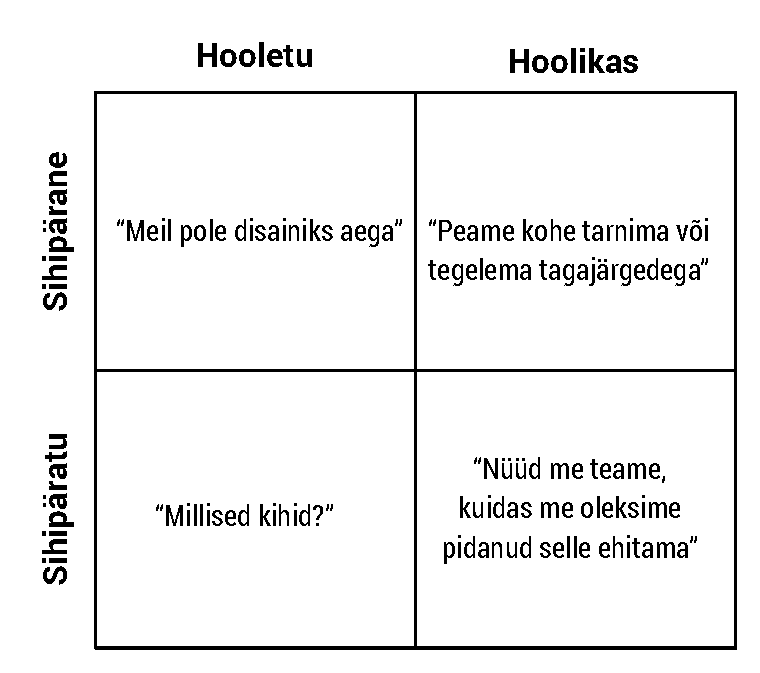
\includegraphics[width=.65\textwidth]{fowler.pdf}
	\end{center}
	\cite{fowlerdebt}
	\note{It is really crucial to understand how much debt you have in each quadrant. \par "no time": high interest loan for fast risky projects \par "what layers?": payday loan \par "Must deliver": trade finance \par "Now we know": mortgage. Difficult to avoid and thus must be used to the max}
\end{frame}

%Arutelu koht
\begin{frame}[fragile]
  \frametitle{Discussion point}
		\begin{center}
			\textbf{How to describe the technical debt to the management?}
		\end{center}
\end{frame}

\section{IT governance}

\begin{frame}[fragile]
  \frametitle{IT governance}
  Essentially the administrative part of IT management
	\begin{itemize}
		\item ITGI definition: ... is an integral part of enterprise governance and consists of the leadership and organisational structures and processes that ensure that the organisation's IT sustains and extends the organisation's strategies and objectives. \citep{insitute2003board}
		\item There is no single good definition, the others also mostly talk about processes and structures
		\note{A nuanced concept: leadership, management, governance\\}
		\item It's all about keeping things under control and moving in a desired direction
	\end{itemize}
	\note{Look, I'm not going to be able to teach you to govern people in a few hours. Thus let's talk about some fundamental forces at play\\}
\end{frame}

\begin{frame}[fragile]
  \frametitle{Policy resistance}
  The tendency of some systems to resist attempts to change their state by not changing, changing in a different direction or return to the original state
	\begin{itemize}
		\item It is a fundamental behaviour of certain dynamic systems, the behaviour of people must be separated from that of the system
		\item Every system is in a sort of equilibrium. The balance might be stable, unstable or neutral
		\item Before imposing any policy or rule on an organisation, always ask
		\begin{itemize}
			\item In this context, what kind of balance is my system in?
			\item What mechanisms will try to resist the policy?
	\end{itemize}

	\end{itemize}
\end{frame}
\note{Example of wolves and rabbits. You need to add rabbits to increase the number of wolves. But how do you add rabbits?}

%Arutelu koht
\begin{frame}[fragile]
  \frametitle{Discussion point}
		\begin{center}
			\textbf{What's the fundamental distinction between \\IT management and IT governance?}
		\end{center}
\end{frame}

\begin{frame}[fragile]
  \frametitle{So what do we govern?}
	What do we govern when we govern IT
	\begin{itemize}
		\item People
		\item Resources
		\item Processes
	\end{itemize}
	\note{This is true for all governance, not just IT}
\end{frame}



\begin{frame}[fragile]
  \frametitle{People}
  People behave in a way that \emph{maximises their interests}. How these interests align with the interests of the company is a management problem
	\begin{itemize}
		\item Again a fundamental problem, not an issue with particular people
		\item This is where a lot of policy resistance stems from 
		\item Before deciding to manage or control people, always ask:
		\note{These must be asked not generally but particularly: Is Steve going to leave?\par}
			\begin{itemize}
				\item Who will leave (or become unhappy). These kind of people you'll lose and \emph{and will not be able to hire and retain again}
				\item Who will be successful. These people will prosper and such \emph{kind of people will multiply}
				\note{Focus on these two groups: how do you like getting less of the first and more of the second?}
			\end{itemize}
		\item \cite{spolsky2008more} covers neatly ways of managing people in an IT context
	\end{itemize}
\end{frame}

\begin{frame}[fragile]
  \frametitle{Resources}
  	All resources are given to the head of IT to \emph{achieve a business objective}. Thus two important questions arise:
		\note{Both questions must be answered the same way by both sides\\}
	\begin{itemize}
		\item What is that objective?
		\item Is the objective achievable with the resources?
		\note{To what extent, actually. Resources are always limited\\}
	\end{itemize}

	Therefore:
	\begin{itemize}
		\item The IT head must maximise the \emph{bang per buck} 
		\note{Anything else is irrelevant. This is why it is crucial to understand what "bang" means in your context\\}
		\item Management of technical debt must be transparent. Paying the debt takes resources and objectives can be achieved by taking on debt
		\note{So why are you paying your debt instead of working on the objectives?}
	\end{itemize}
\end{frame}


\begin{frame}[fragile]
  \frametitle{Processes}
	\begin{itemize}
		\item Process governance is a classic feedback control problem of cybernetics. Input is given, the output is measured, measurement is compared to the desired value, input is adjusted
		\note{In Greek. kybernetike "governance"\\}
		\item Typically the quality of out put and the cost are measured
		\item As the modern world cannot usually be micromanaged, the key question becomes \emph{how to scale process control up?} 
		\item Spear \citep{spear2010high} claims doing this allows for differentiation and competitive advantage
		\note{Spear is very good\\}
		\item The Japanese currently have the most sensible model for answering the question. See \emph{Kaizen, muda/mura/muri}
		\note{Agile methods follow the same approach in many ways and are also rooted in the car industry (the 3c project)}
	\end{itemize}
\end{frame}


%Arutelu koht
\begin{frame}[fragile]
  \frametitle{Discussion point}
		\begin{center}
			\textbf{Why and how can the output of a programmer be measured?}
		\end{center}
\end{frame}

\begin{frame}[fragile]
  \frametitle{Managing IT input}
  \begin{center}
	  The problem: \textbf{How to decide in which order\\ the customer needs are met?}
		\\[3mm]
	\emph{There is, by definition, always less resources than needs}
  \end{center}
\end{frame}
\note{Although the issue is mostly tactical, it is a problem area for many organisations. Thus the slight detour}
    
\begin{frame}[fragile]
  \frametitle{The project list grows}
  If the pool is filled faster than the water flows out, water levels rise
		\begin{itemize}
			\item The longer the queue (the more water in the pool), the slower the organisation
			\note{If our pool contains three years worth of projects, the last one will be implemented in three years even if all the needs are met as fast as they occur\\}
			\item There must exist a sensible way to manage the queue
			\note{For example, the queue is defined to be of fixed size: if something is added, something else drops off\\}
			\item "The paperwork block" is a bad idea as this drives up the cost of dropping off the list
			\item The projects have a tendency to go sour while waiting
			\item "Buffer bloat" is a very similar issue in nature
		\end{itemize}
\end{frame}

\begin{frame}[fragile]
  \frametitle{Inevitable political pressure}
  	There is an inevitable pressure to bypass any mechanism of governing limited resources
		\begin{itemize}
			\item Decisions must be very transparent and preferably consensual 
			\item It is a good idea to remove humans from the loop altogether by defining simple mechanical rules
			\note{For example: every unit gets x amount of developer hours. No more, no less\\}
			\item The lower in organisation the decisions, the less political pressure there is
			\note{The decisions should be pushed to the lowest level where both sides could have experienced well-mandated people reaching an agreement\\}
			\item The more frequent the decisions, the easier they are to make
			\note{50 projects in 5 hours or 5 one-hour meeting each with 10 projects. Ad-hoc decisions are thus preferred\\}
			\item There must be a sensible and accepted way to make exceptions without discrediting the process
			\note{For example, "the grandfather principle"}
		\end{itemize}
\end{frame}

\begin{frame}[fragile]
  \frametitle{Important stuff might not get done}
		\begin{itemize}
			\item There must exist a way to get small important stuff done fast 
			\item Because it is usually almost impossible to push technical debt payment through the decision process
			\item Technical debt is the pain of IT and not the business. It is only perceived as decline in deliveries that can easily be attributed to incompetence
			\item The bigger the "stones"
			\begin{itemize}
				\item The more efficient decision-making is
				\note{Efficiency is an immediate problem while its causes are strategic and long-term in nature\\}
				\item The bigger the stakes and the more fierce the fighting
				\item The more space between the stones, the less efficient the process
				\item The slower the organisation
				\note{See the note on pushing decisions down, i.e. making them smaller}
			\end{itemize}
		\end{itemize}
\end{frame}


%Arutelu koht
\begin{frame}[fragile]
  \frametitle{Discussion point}
		\begin{center}
			\textbf{What to do when the customer does not listen?}
		\end{center}
\end{frame}



\begin{frame}[t,allowframebreaks,]
  	\bibliographystyle{plainnat}
	\bibliography{it_strateegia} 

\end{frame}

%\plain{Küsimusi?}
\plain{Questions?}
\end{document}